\newpage
\hypertarget{finalStep}{}
\section{Tree-to-text transformation}
\genHeader

We've finally reached the last step, transforming our tree result, \texttt{fwd.trg.xmi} back into a filesystem with \texttt{.dictionary} files identical to our
original input, the \texttt{myLibrary} filesystem.

Note that in an actual application, we would do something useful with the model before transforming it back to text, or the dictionary might have been produced
from a learning box, i.e., the textual syntax representation wouldn't exist yet. One of the coolest things about ANTLR is that the same parsing technology that
we used in Section 2 can be used to \emph{unparse} the tree.

Analogously to parsing text with a lexer and parser grammar to produce a tree, a tree is unparsed to text using a \emph{tree grammar} and \emph{templates}. A
tree grammar is similar to EBNF, consisting of rules (\texttt{main}, \texttt{entry}) that each match a tree fragment and evaluate a template, as
opposed to rules that match text fragments and build a tree. For further details concerning tree grammars, we refer to \cite{ANTLR} and the ANTLR
website \url{www.antlr.org}.

\begin{itemize}

\item[$\blacktriangleright$] Expand ``src/org.moflon.moca.dictionary.unparser'', open \texttt{Dict\-ion\-ary\-Tree\-Gram\-mar.g}, and edit the contents as
depicted in Fig.~\ref{eclipse:treeGrammar}. 

\vspace{0.5cm}

\item[$\blacktriangleright$] Next, open \texttt{Dict\-ion\-ary\-Un\-pars\-er\-Ad\-ap\-ter.java} (Fig~\ref{eclipse:unparserCommented}). You'll notice that this
file contains a (commented) \texttt{StringTemplateGroup} meth\-od for retrieving a group of templates and needs to be implemented. The comments explain how to
use either a folder containing different template files, or a single file containing all templates. The latter is better for numerous small templates, while the
former makes sense when the templates contain a lot of static text.

\vspace{0.5cm}

\item[$\blacktriangleright$] For this small example, a single file with all templates is ideal. Uncomment line 44 (the option for a group file) and remove
the line throwing an \texttt{Un\-sup\-port\-ed\-Op\-er\-at\-ion\-Ex\-cep\-tion}.

\newpage 

\vspace*{2cm}

\begin{figure}[htpb]
\begin{center}
  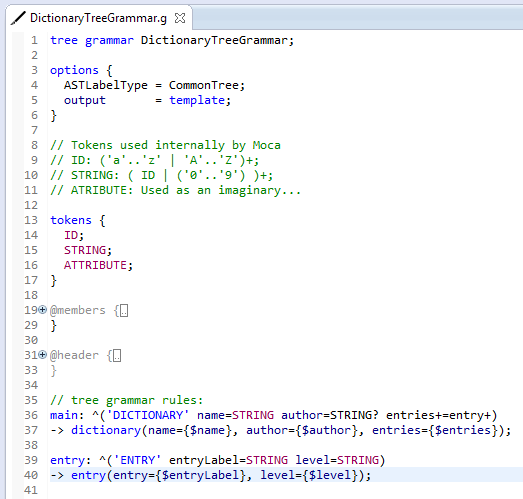
\includegraphics[width=0.8\textwidth]{eclipse_dictionaryTreeGrammar}
  \caption{Tree grammar for the unparser}
  \label{eclipse:treeGrammar}
\end{center}
\end{figure}

\vspace{1cm}

\begin{figure}[htpb]
\hspace{-1cm}
  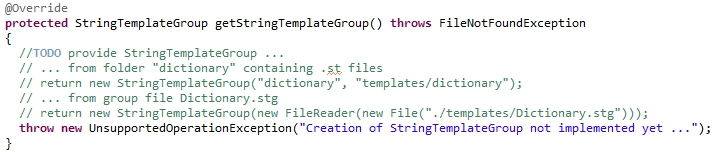
\includegraphics[width=1.2\textwidth]{eclipse_DictionaryUnparserAdapterUnimplemented}
  \caption{Two options of how to store templates}
  \label{eclipse:unparserCommented}
\end{figure}

\newpage


\item[$\blacktriangleright$] Create a template file by navigating to the empty ``templates'' folder of your adapter project, and creating a new file
named \texttt{Dictionary.stg} (as demanded in \texttt{Dict\-ion\-ary\-Un\-pars\-er\-Ad\-ap\-ter.java}). Complete it as specified in
Fig.~\ref{eclipse:dictionaryTemplate}.

\vspace{0.5cm}

\begin{figure}[htpb]
\begin{center}
  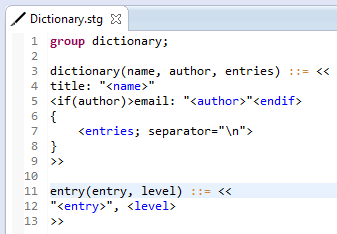
\includegraphics[width=0.5\textwidth]{eclipse_dictionaryTemplate}
  \caption{The \texttt{dictionary} template}
  \label{eclipse:dictionaryTemplate}
\end{center}
\end{figure}

\item[$\blacktriangleright$] Copy and paste \texttt{fwd.trg.xmi} into ``instances," naming the new file \texttt{bwd.src.xmi}. This will be the backward
transformation's input file.

\item[$\blacktriangleright$] Save and run your transformation again -- there should no longer be an error message in the console. Inspect and compare your input
and output folders and their containing files (Fig.~\ref{eclipse:unparseResult}). Are they the same?

\vspace{0.5cm}

\begin{figure}[htpb]
\begin{center}
  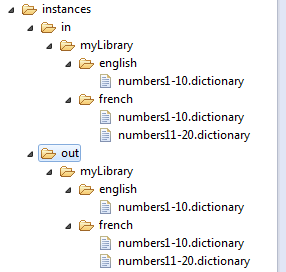
\includegraphics[width=0.4\textwidth]{eclipse_finalInstancesHierarchy}
  \caption{The final input and output filesystems}
  \label{eclipse:unparseResult}
\end{center}
\end{figure}

\item[$\blacktriangleright$] If everything succeeded, your transformation is now complete in both directions! Feel free to play around with
changing some files such as a the unparser template, or the content of the original files. How are the changes propagated through the transformation?
How about implementing an SDM to refactor or extend the library model in some useful way before transforming it to text?

\end{itemize}